\documentclass[times, utf8, zavrsni]{fer}
\usepackage{booktabs}
\usepackage{listings}
\usepackage{listings}
\usepackage{color}
\definecolor{lightgray}{rgb}{.9,.9,.9}
\definecolor{darkgray}{rgb}{.4,.4,.4}
\definecolor{purple}{rgb}{0.65, 0.12, 0.82}

\lstset{language=SQL,
  belowskip=3mm,
  breakatwhitespace=true,
  breaklines=true,
  classoffset=0,
  columns=flexible,
  commentstyle=\color{dkgreen},
  framexleftmargin=0.25em,
  keywordstyle=\color{blue},
  numbers=none, %If you want line numbers, set `numbers=left`
  numberstyle=\tiny\color{gray},
  showstringspaces=false,
  stringstyle=\color{mauve},
  tabsize=3,
  xleftmargin =1em
}

\lstdefinelanguage{JavaScript}{
  keywords={typeof, new, true, false, catch, function, return, null, catch, switch, var, if, in, while, do, else, case, break, const, let, async},
  keywordstyle=\color{blue}\bfseries,
  ndkeywords={class, export, boolean, throw, implements, import, this},
  ndkeywordstyle=\color{darkgray}\bfseries,
  identifierstyle=\color{black},
  sensitive=false,
  comment=[l]{//},
  morecomment=[s]{/*}{*/},
  commentstyle=\color{purple}\ttfamily,
  stringstyle=\color{red}\ttfamily,
  morestring=[b]',
  morestring=[b]"
}

\lstset{
   language=SQL,
   extendedchars=true,
   basicstyle=\footnotesize\ttfamily,
   showstringspaces=false,
   showspaces=false,
   numbers=none,
   numberstyle=\footnotesize,
   numbersep=9pt,
   tabsize=2,
   breaklines=true,
   showtabs=false,
   captionpos=b
}

\lstset{
   language=JavaScript,
   extendedchars=true,
   basicstyle=\footnotesize\ttfamily,
   showstringspaces=false,
   showspaces=false,
   numbers=left,
   numberstyle=\footnotesize,
   numbersep=9pt,
   tabsize=2,
   breaklines=true,
   showtabs=false,
   captionpos=b
}

\lstset{
     literate=%
         {á}{{\'a}}1
         {í}{{\'i}}1
         {é}{{\'e}}1
         {ý}{{\'y}}1
         {ú}{{\'u}}1
         {ó}{{\'o}}1
         {đ}{{\'đ}}1
         {ě}{{\v{e}}}1
         {š}{{\v{s}}}1
         {č}{{\v{c}}}1
         {ř}{{\v{r}}}1
         {ž}{{\v{z}}}1
         {ď}{{\v{d}}}1
         {ť}{{\v{t}}}1
         {ň}{{\v{n}}}1
         {ů}{{\r{u}}}1
         {Á}{{\'A}}1
         {Í}{{\'I}}1
         {É}{{\'E}}1
         {Ý}{{\'Y}}1
         {Ú}{{\'U}}1
         {Ó}{{\'O}}1
         {Ě}{{\v{E}}}1
         {Š}{{\v{S}}}1
         {Č}{{\v{C}}}1
         {Ř}{{\v{R}}}1
         {Ž}{{\v{Z}}}1
         {Ď}{{\v{D}}}1
         {Ť}{{\v{T}}}1
         {Ň}{{\v{N}}}1
         {Ů}{{\r{U}}}1
}

\begin{document}

% TODO: Navedite broj rada.
\thesisnumber{920}

% TODO: Navedite naslov rada.
\title{Web-aplikacija za praćenje podataka o nogometnim utakmicama}

% TODO: Navedite vaše ime i prezime.
\author{Marko Jerkić}

\maketitle

% Ispis stranice s napomenom o umetanju izvornika rada. Uklonite naredbu \izvornik ako želite izbaciti tu stranicu.
% TODO: Treba li mi izbornik?
% \izvornik

% Dodavanje zahvale ili prazne stranice. Ako ne želite dodati zahvalu, naredbu ostavite radi prazne stranice.
\zahvala{}

\tableofcontents

\chapter{Uvod}

Nogomet je najpopularniji sport na svijetu i postoji velika zainteresiranost za praćenje rezultata nogometnih utakmica.
Nekoć su se rezultati utakmica mogli vidjeti tek dan nakon u novinama i časopisima, ali mi danas živimo u doba interneta.

Ljudi žele vidjeti rezultate utakmica na što lakši način i na svojim mobilnim uređajima i računalima.
Novine su nekoć donosile rezultate prošlih utakmica, najave utakmica za naredni dan te za neke bitnije utakmice bi opisali ukratko najznačajnije trenutke.
Internet nam je omogućio da se podatci utakmica mogu držati u jednoj središnjoj bazi podataka, a korisnik može pristupiti tim podatcima kada kod hoće.

To znači da izradom odgovarajućeg korisničkog sučelja i potrebnih API-ja možemo omogućiti korisniku pretraživanje ekipa, igrača i utakmica koje ga zanimaju godinama unazad, dok su novine pisale samo o onim utakmicama koje su bile aktualne u to vrijeme.

Pored toga, možemo prikazati puno više podataka i detalja koji bi korisnika mogle zanimati.
Neke od stvari koje bi korisnika mogle zanimati su: igrači koji su zabili golove, grafički prikaz početnih postava domaće i gostujuće ekipe, detaljna statistika utakmice, tablice poretka u natjecanju i slično.

Internet nam također omogućuje ažuriranje podataka o utakmici u stvarnom vremenu koristeći protokol WebSockets\footnote{https://developer.mozilla.org/en\-US/docs/Web/API/WebSockets\_API}.
Korisnik tada ne mora ponovo učitati stranicu da bi dobio najnovije podatke.

U prva dva poglavlja ovoga rada napravljena je analiza postojećih rješenja na internetu i odabir glavnih funkcionalnosti koje se planiraju izraditi u sklopu projekta.
Dalje slijedi opis modela baze podataka. Tu su opisani svi entiteti i njihove veze. Nakon toga dolazi poglavlje koje opisuje arhitekturu aplikacije, odabrane tehnologije i korištene biblioteke.
Zatim je opisan process izrade aplikacije opisujući sve izrađene funkcionalnosti. Na kraju dolazi zaključak koji opisuje rezultat projekta.

\chapter{Analiza postojećih rješenja na internetu}
Za analizu postojećih rješenja na internetu su korištene aplikacije Sofascore\footnote{https://sofascore.com}, OneFootball\footnote{https://onefootball.com} i Rezultati.com\footnote{https://rezultati.com}.

\section{Prikaz liste utakmica}

Jedan od glavnih dijelova aplikacija koje se koriste za praćenje nogometnih rezultata je stranica pregleda popisa dostupnih utakmica.
Većina postojećih rješenja na internetu koriste ovu stranicu kao središnju lokaciju s koje se pregleda većina sadržaja. To je istina za aplikacije Sofascore i Rezultati.com.

U slučaju te dvije aplikacije, prilikom pristizanja na samu web-lokaciju, prikazana nam je lista postojećih utakmica koje se igraju na dan posjećivanja aplikacije.

Središnja komponenta početne stranice Sofascore-a je lista utakmica grupirana po natjecanjima i državama. Prvih nekoliko prikazanih natjecanja su istaknuta ili spremljena natjecanja.
U slučaju kada korisnik prvi put posjećuje stranicu ili nema spremljenih podataka u pregledniku, istaknuta natjecanja uključuju velika svjetska natjecanja,
kao engleska Premier liga, njemačka Bundesliga i slično te velika natjecanja u državi iz koje korisnik posjećuje stranicu.
Za korisnika koji posjećuje stranicu iz Hrvatske, među istaknutim natjecanjima se nalazi Hrvatska nogometna liga.
Nakon istaknutih natjecanja, prikazuju se natjecanja iz cijelog svijeta koja sadrže utakmice za odabrani dan. Natjecanja su grupirana po državama u kojima se održava to natjecanje.

Osim popisa utakmica, koji se nalazi u sredini aplikacije, Sofascore sadrži kalendar s lijeve strane popisa utakmica.
Kalendar se koristi za odabir datuma prema kojemu se prikazuju dostupne utakmice.
Ispod kalendara se nalazi popis istaknutih natjecanja i popis svih dostupnih natjecanja s poljem za unos teksta koji se koristi za sužavanje izbora.

S desne strane popisa utakmica se nalazi pretpregled istaknute utakmice. Pretpregled sadrži ime i grb ekipa koje sudjeluju u utakmici te rezultat utakmice.
Ispod toga se nalazi popis istaknutih igrača te reklame za sportsko klađenje.

Aplikacija Rezultati.com ima dosta sličan raspored na početnoj stranici, ali ne prikazuje istaknuta natjecanja, utakmice niti igrače.
Aplikacija OneFootball ne koristi popis dostupnih utakmica na početnoj stranici. OneFootball je aplikacija koja se fokusira prvenstveno na nogometne novosti.
Do stranice na kojoj se prikazuje popis dostupnih utakmica se dolazi preko poveznice koja se nalazi na navigacijskoj traci.

\section{Prikaz detalja utakmice}

Sve tri aplikacije koje su korištene za analizu postojećih rješenja imaju dosta različito ponašanje prilikom odabira utakmice s popisa.
Prilikom odabira utakmice na aplikaciji Sofascore otvori se pretpregled desno od popisa utakmica.
Aplikacija Rezultati.com otvori detalje utakmice u skočnom prozoru, dok OneFootball otvori novu stranicu.

Zaglavlje stranice detalja utakmice prikazuje ime i grb ekipa koje sudjeluju u utakmici, datum utakmice i trenutni rezultat.
Detaljni podatci su raspodijeljeni u više kategorija koje se odabiru preko kartica. Zadana kartica sadrži događaje utakmice, kao što su pogodci, kartoni i zamjene, kronološki poredane po minuti.

\begin{figure}[htb]
\centering
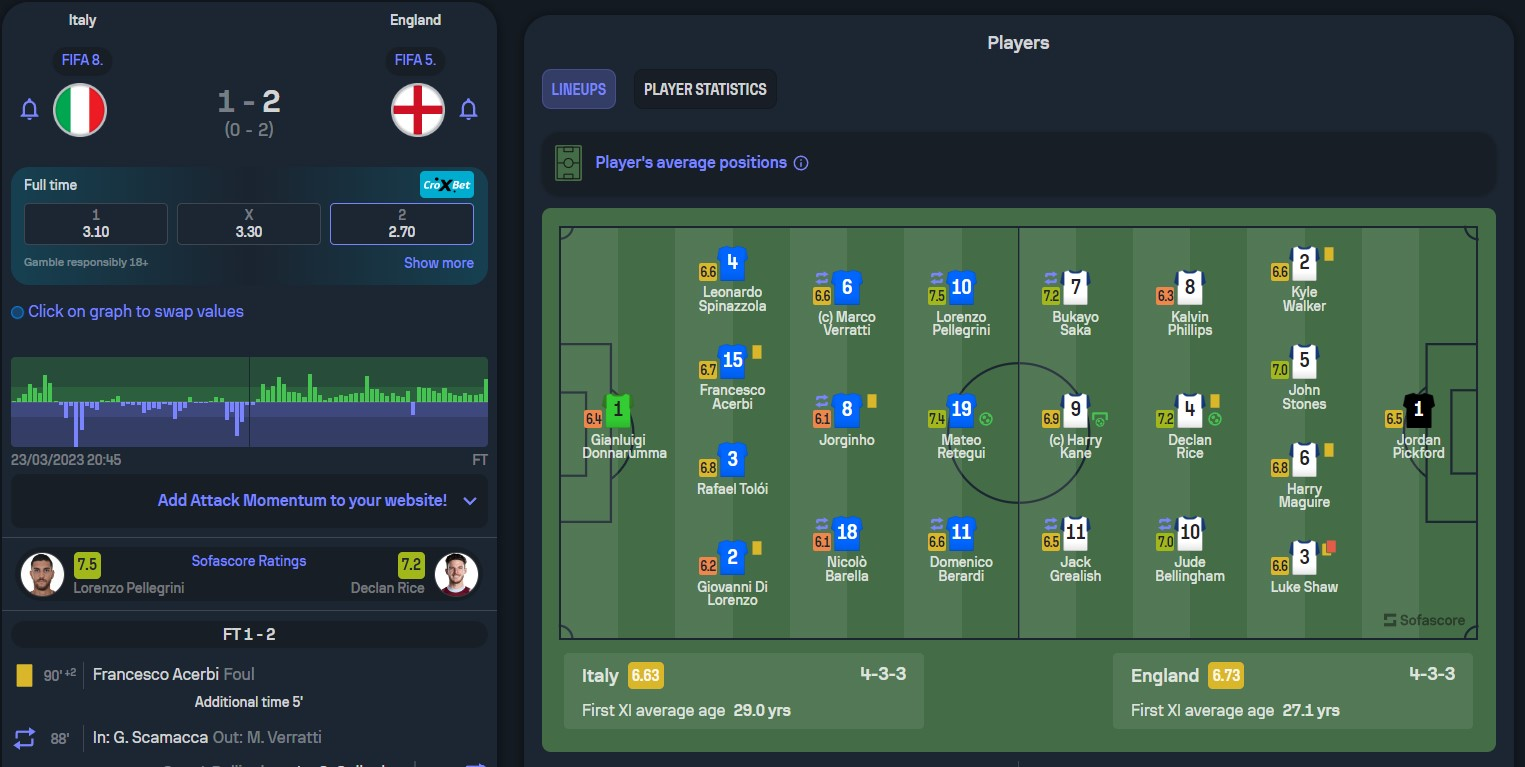
\includegraphics[width=15cm]{images/ss-detail.jpg}
\caption{Detalji utakmice na SofaScore}
\label{fig:ss-detail}
\end{figure}

Pored kartice događaja po minuti, bitne su još kartica početnih postava dviju ekipa te kartica statistike utakmice.
Kartica početnih postava utakmice grafički prikazuje prvih jedanaest igrača obje ekipe, formaciju, boju dresova te broj na dresovima.
Kartica statistike prikazuje podatke o posjedu lopte, broju udaraca, broju udaraca u vrata, broju udaraca iz kuta i sl., za obje ekipe.


\section{Prikaz detalja igrača, izbornika, ekipa i natjecanja}

Nakon stranica prikaza popisa utakmica i detalja pojedinačne utakmice, sporednu ulogu u odabranim aplikacijama zauzimaju stranice pregleda detalja igrača, izbornika, ekipa i natjecanja.

Stranice pregleda detalja igrača i izbornika su dosta slične. Obje prikazuju ime osobe, sliku, datum rođenja i nacionalnost.
Ispod toga se prikazuju kartice s popisom najnovijih utakmica u kojima je sudjelovala ta osoba, osobna statistika te popis ekipa za koje je ta osoba igrala ili koje je ta osoba trenirala.

Stranica prikaza detalja o ekipi prikazuje ime ekipe, grb i državu iz koje dolazi. Nakon toga se prikazuju kartice s podatcima o nedavnim utakmicama koje je igrala ekipa,
trenutnim igračima koji igraju za tu ekipu, te tablica poretka natjecanja u kojemu ta ekipa sudjeluje.

Kod stranice pregleda natjecanja, najbitnije su kartice s tablicom poretka te popisom utakmica po sezoni za odabrano natjecanje.

\chapter{Cilj izrade projekta}

Nakon analize postojećih rješenja na internetu izdvojene su određene funkcionalnosti koje se čine najbitnije i najkorisnije prosječnom korisniku.
Najbitnija funkcionalnost aplikacije za pregled rezultata utakmica je detaljni prikaz podataka utakmice.
Detaljni prikaz podataka utakmice mora sadržavati rezultat utakmice, događaje utakmice, početne postave te statistiku.

Događaji utakmice moraju sadržavati popis golova, zamjena i podijeljenih kartona. Svi događaji moraju biti poredani silazno prema minuti utakmice u kojoj je došlo do tog događaja.
Za svaki gol mora se prikazati tko ga je postigao, tko je asistirao, koji je rezultat utakmice bio nakon tog pogotka te u kojoj minuti je zabijen.
Imena igrača koji su zabili ili asistirali za taj gol moraju biti poveznice koje će korisnika odvesti na stranicu pregleda detalja o tom igraču.
Pored kartona mora pisati ime igrača koji ga je dobio.
Treba grafički prikazati je li karton žuti, crveni ili drugi žuti.
Zamjena mora prikazati ime igrača koji ulazi u igru te ime igrača koji izlazi iz igre.
Imena igrača koji su dobili karton ili su sudjelovali u zamjeni također moraju biti poveznice koje vode na stranicu detalja igrača.

Stranica pregleda početnih postava ekipa mora grafički prikazati koja se formacija koristi te u odgovarajućoj formaciji prikazati dres igrača s njegovim brojem koji nosi na utakmici te ime igrača.
Svaki dres koji predstavlja igrača u početnoj postavi mora biti poveznica na stranicu pregleda detalja igrača.
U slučaju kada početne postave ekipa koje sudjeluju u određenoj utakmici nisu dostupne, potrebno je obavijestiti korisnika o nedostatku podataka i prikazati popis igrača koji su dostupni odabranoj ekipi za tu sezonu.

Potrebno je omogućiti prikaz svih dostupnih utakmica za odabrani datum. Svaka prikazana utakmica mora sadržavati ime domaće i gostujuće ekipe, vrijeme održavanja utakmice te rezultat.

Korisnik mora moći pretražiti dostupne igrače, trenere i ekipe. Rezultati pretrage moraju biti poveznice na detaljni pregled podataka odabranog entiteta.

Kod pregleda detalja igrača i trenera potrebno je prikazati osnovne informacije kao ime, prezime i sliku osobe ako je dostupna.
Potrebno je prikazati trenutnu ekipu kojoj igrač ili trener pripada te popis ekipa kojima je pripadao u određenoj sezoni.
Treba se omogućiti prikaz utakmica u kojima je sudjelovao odabrani trener ili igrač.

Potrebno je omogućiti prijavu i registraciju korisnika. Prijavljeni korisnik treba imati mogućnost spremanja najdražih igrača i ekipa kako bi brže došao do podataka koji ga zanimaju.
Korisnik koji ima ulogu administratora treba imati mogućnost uređivanja i unosa novih podataka za odabrani set entiteta.

\chapter{Model baze podataka}

Dizajnirani relacijski model podataka sadrži 18 tablica te četiri enumerirane vrste podataka.

\section{Model entiteti-veze}

Svi izrađeni entiteti imaju UUID identifikator koji skuži kao primarni ključ.
Središnji entitet relacijskog modela je tablica "Game," koja sadrži osnovne podatke o utakmici.
Ovaj entitet sadrži alternativni ključ na natjecanje kojemu pripada utakmica, domaću i gostujuću ekipu, izbornika domaće i gostujuće ekipe,
sezonu u kojoj se igra utakmica te na entitet koji sadrži detaljniju statistiku utakmice.
Tablica "Game" sadrži alternativni ključ na entitet "GameStatistic," ali taj podatak nije obavezan jer svaka utakmica ne mora imati podatke o statistici.
U slučaju kada utakmica još nije počela, entitet "Game" ne sadrži podatke o statistici pa to polje sadrži vrijednost \emph{null}.

\begin{figure}[htb]
\centering
\includegraphics[width=14cm]{images/erd-min.png}
\caption{ERD dijagram baze podataka}
\label{fig:hero}
\end{figure}

Entitet "Game" također sadržava informaciju o vremenu početka utakmice, vremenu nadoknade u prvom i drugom poluvremenu, boju dresova domaće i gostujuće ekipe spremljenu kao heksadecimalna vrijednost,
kao i boje dresova vratara, status utakmice, te početne postave dviju ekipa.
Status utakmice se sprema kao enumerirana vrijednost koja može poprimiti vrijednosti "NOT\textunderscore STARTED," "STARTED," "HALFTIME" te "OVER".

Početne postave prvih jedanaest se spremaju kao "jsonb"\footnote{https://www.postgresql.org/docs/9.5/functions-json.html} \citep{postgressjson} vrsta podataka.
Podatci se spremaju kao JSON polje od jedanaest vrijednosti koje predstavljaju jedanaest igrača početne postave.
U tom JSON podatku je spremljen identifikator igrača, broj dresa koji igrač nosi na toj utakmici, broj reda u početnoj formaciji te redni broj igrača u tome redu gledajući s lijeva na desno.
Odlučeno je spremati početnu postavu kao JSON vrijednost umjesto da se stvori novi entitet koji bi imao vezu na entitet "Game" jer bi to stvorilo previše unosa u bazi podataka, točnije 22 po svakoj spremljenoj utakmici.
Pored toga, spremanje tog podatka kao JSON je olakšalo način izrade administracije početne postave kroz klijentsku aplikaciju.

Entitet "GameStatistics" sadrži podatke kao što su ukupni udarci, udarci u vrata, ubačaji iz kuta, prekršaji, stvorene velike prilike, broj dodavanja, broj ubacivanje lopte u šesnaesterac, broj driblinga i broj uklizavanja za obje ekipe.

Pored nabrojanih podataka iz entiteta "GameStatistics," izdvojeni su podatci o zabijenim pogotcima, podijeljenim kartonima te zamjenama kao posebni entiteti.
Razlog tomu je taj što svi ovi podatci sadrže bar jednu vezu na nekog igrača.
Entitet "Goal" sadrži podatak o igraču koji je zabio pogodak, o igraču koji je asistirao te vrijeme u minutama kada je zabijen pogodak.
Entitet "CardAwarded" sadrži igrača koji je dobio karton, minutu u kojoj je igrač dobio karton, te vrstu kartona koji je dodijeljen.
A entitet "Substitution" sadrži igrača koji je izašao s terena, igrača koji ulazi u teren te minutu u kojoj je zamjena izvršena.
Sva tri navedena entiteta imaju alternativni ključ na utakmicu kojoj pripadaju.

Svaka utakmica pripada jednom natjecanju u određenoj sezoni.
Entitet "Competition" sadrži ime, podatak o državi u kojoj se igra te podatak o tome je li to natjecanje označeno kao istaknuto.
Država u kojoj se igra natjecanje je spremljena kao poseban entitet koji sadrži naziv države te poveznicu na sličicu zastave te države.
Svako natjecanje može imati više sezona, te za jednu sezonu može postojati više natjecanja.
Sezona je spremljena kao vlastiti entitet i jedini podatak koji sadrži, pored identifikatora, je naziv te sezone.

Entitet "Team" sadrži podatke o nazivu ekipe, državi iz koje potječe ekipa te URL adresu sličice grba ekipe.
Entitet "Team" sadrži više-na-više vezu s poveznom tablicom "CompetitionInSeason" koja sadrži vezu na jedno natjecanje i sezonu.

Entiteti "Manager" i "Player" su dosta slični. Oba sadrže ime, prezime, datum rođenja, alternativni ključ na trenutnu ekipu (koja nije obavezna) te alternativni ključ na entitet "Country" koji predstavlja nacionalnost osobe.
Oba imaju više-na-više vezu s poveznom tablicom "TeamInCompetition" koja sadrži podatak o ekipi koja igra u određenom natjecanju u određenoj sezoni.
To znači da jedan trener ili igrač može pripadati većem broju ekipa u jednoj sezoni, ali također ne mora pripadati niti jednoj ekipi za određenu sezonu.

Pored nabrojanih entiteta postoje još entiteti potrebni za autentifikaciju te spremanje najdražih igrača i ekipa korisnika.

\section{Relacijski model podataka}

Model baze podataka sadrži četiri enumerirana tipa.
\begin{lstlisting}[caption=Enumerirani tipovi, language=SQL, numbers=none]

-- Vrsta kartona kojeg igrač može dobiti
create type "CardType" as enum ('RED', 'YELLOW', 'SECOND_YELLOW');
-- Status utakmice
create type "Halftime" as enum ('FIRST_HALF', 'SECOND_HALF', 'EXTRA_FIRST_HALF', 'EXTRA_SECOND_HALF');
-- Uloga korisnika
create type "UserRole" as enum ('USER', 'ADMIN');
-- Status utakmice
create type "GameStatus" as enum ('NOT_STARTED', 'STARTED', 'HALFTIME', 'OVER');

\end{lstlisting}

Dalje slijede naredbe potrebne za stvoriti relacijski model baze podataka.
\begin{lstlisting}[caption=Model baze podataka, language=SQL, numbers=none]
-- Registrirani korisnik
create table if not exists "User"
(
    id          text       not null primary key,
    "firstName" text       not null,
    "lastName"  text       not null,
    email       text       not null,
    role        "UserRole" not null
);

-- Trener
create table if not exists "Manager"
(
    id          text not null primary key,
    "firstName" text not null,
    "lastName"  text not null,
    "teamId"    text,
    "imageSlug" text,
    unique ("teamId")
);

-- Sezona
create table if not exists "Season"
(
    id          text    not null primary key,
    title       text    not null,
    "isCurrent" boolean not null,
    unique (title)
);

-- Država
create table if not exists "Country"
(
    id          text not null primary key,
    name        text not null,
    "imageSlug" text,
    unique (name)
);

create table if not exists "Player"
(
    id                   text         not null primary key,
    "firstName"          text         not null,
    "lastName"           text         not null,
    "primaryShirtNumber" integer,
    "primaryPosition"    "Position"   not null,
    "dateOfBirth"        timestamp(3) not null,
    "imageSlug"          text,
    "countryId"          text         not null
        references "Country"
            on update cascade on delete restrict,
    "teamId"             text
);

-- Veza korisnika i igrača koji je spremljen kao favorit
create table if not exists "FavouritePlayer"
(
    id         text not null primary key,
    "userId"   text not null
        references "User"
            on update cascade on delete restrict,
    "playerId" text not null
        references "Player"
            on update cascade on delete restrict
);

-- Natjecnje, npr. Premier liga
create table if not exists "Competition"
(
    id              text              not null primary key,
    name            text              not null,
    "countryId"     text              not null references "Country"
            on update cascade on delete restrict,
    "isHighlighted" boolean           not null,
    "imageSlug"     text,
);

-- Veza natjecanja i sezone
-- Npr. Premier liga u sezoni 2018./19.
create table if not exists "CompetitionInSeason"
(
    id text not null primary key,
    "competitionId" text not null references "Competition"
            on update cascade on delete restrict,
    "seasonId"      text not null references "Season"
            on update cascade on delete restrict
);

-- Ekipa, npr. Liverpool
create table if not exists "Team"
(
    id text not null primary key,
    name                text not null,
    "countryId"         text not null references "Country"
            on update cascade on delete restrict,
    "imageSlug"         text,
    "groupId"           text,
    "primaryShirtColor" text not null
);

-- Veza korisnika i ekipe koja je označena kao najdraža
create table if not exists "FavouriteTeam"
(
    id       text not null primary key,
    "userId" text not null references "User"
            on update cascade on delete restrict,
    "teamId" text not null references "Team"
            on update cascade on delete restrict
);

-- Veza igrača, ekipe i sezone
-- Npr. Lovren je igrao u Liverpool-u u sezoni 2018./19.
create table if not exists "PlayersTeamInSeason"
(
    id         text not null primary key,
    "teamId"   text not null references "Team"
            on update cascade on delete restrict,
    "playerId" text not null references "Player"
            on update cascade on delete restrict,
    "seasonId" text not null references "Season"
            on update cascade on delete restrict,
    unique ("teamId", "playerId", "seasonId")
);

-- Veza ekipe, natjecanja i sezone
-- Npr, Liverpool je igrao u Premier ligi u sezoni 2021./22.
create table if not exists "TeamInCompetition"
(
    id              text not null primary key,
    "teamId"        text not null references "Team"
            on update cascade on delete restrict,
    "competitionId" text not null references "Competition"
            on update cascade on delete restrict,
    "seasonId"      text not null references "Season"
            on update cascade on delete restrict
);

-- Ekipa koja je označena kao istaknuta
-- Koristi se za prikaz na početnoj stranici
create table if not exists "HighlightedTeam"
(
    id       text not null primary key,
    "teamId" text not null references "Team"
            on update cascade on delete restrict
);

-- Entitet utakmice
create table if not exists "Game"
(
    id text not null primary key,
    "competitionId" text not null references "Competition"
            on update cascade on delete restrict,
    "homeTeamId" text not null references "Team"
            on update cascade on delete restrict,
    "awayTeamId" text not null references "Team"
            on update cascade on delete restrict,
    "gameStatisticsId" text,
    "kickoffTime" timestamp(3) not null,
    "firstHalfEndedAferAdditionalTime"  integer not null,
    "secondHalfEndedAferAdditionalTime" integer not null,
    "seasonId" text references "Season"
        on update cascade on delete set null,
    "homeTeamShirtColor" text not null,
    "homeTeamGoalkeeperShirtColor" text not null,
    "awayTeamShirtColor" text not null,
    "awayTeamGoalkeeperShirtColor" text not null,
    "homeTeamLineup" jsonb not null,
    "awayTeamLineup" jsonb not null,
    status "GameStatus" default 'OVER'::"GameStatus" not null,
    "awayTeamManagerId" text default 'clh6fsxgu0000uvimeozrkg1m'::text not null
        references "Manager"
            on update cascade on delete restrict,
    "homeTeamManagerId" text default 'clh6fsxgu0000uvimeozrkg1m'::text not null
        references "Manager"
            on update cascade on delete restrict
);

-- Gol koji je zabijen na utakmici
create table if not exists "Goal"
(
    id text not null primary key,
    "scorerId" text not null references "Player"
            on update cascade on delete restrict,
    "isOwnGoal"           boolean not null,
    "isPenalty"           boolean not null,
    "scoredInMinute"      integer not null,
    "scoredInExtraMinute" integer,
    "isHomeTeamGoal"      boolean not null,
    "assistentId"         text references "Player"
            on update cascade on delete set null,
    "gameId" text    not null references "Game"
            on update cascade on delete restrict
);

-- Statistički detalji utakmice
create table if not exists "GameStatistics"
(
    id text not null primary key,
    "homeTeamBallPossession"   integer not null,
    "gameId" text not null references "Game"
            on update cascade on delete restrict,
    "homeTeamTotalShots"       integer not null,
    "homeTeamShotsOnTarget"    integer not null,
    "homeTeamCornerKicks"      integer not null,
    "homeTeamOffsides"         integer not null,
    "homeTeamFouls"            integer not null,
    "homeTeamBigChances"       integer not null,
    "homeTeamPasses"           integer not null,
    "homeTeamCrosses"          integer not null,
    "homeTeamTackles"          integer not null,
    "homeTeamDribles"          integer not null,
    "homeTeamDriblesSucessful" integer not null,
    "awayTeamBallPossession"   integer not null,
    "awayTeamTotalShots"       integer not null,
    "awayTeamShotsOnTarget"    integer not null,
    "awayTeamCornerKicks"      integer not null,
    "awayTeamOffsides"         integer not null,
    "awayTeamFouls"            integer not null,
    "awayTeamBigChances"       integer not null,
    "awayTeamPasses"           integer not null,
    "awayTeamCrosses"          integer not null,
    "awayTeamTackles"          integer not null,
    "awayTeamDribles"          integer not null,
    "awayTeamDriblesSucessful" integer not null,
    unique ("gameId")
);

-- Karton koji je dan na utakmici nekome igraču
create table if not exists "CardAwarded"
(
    id text not null primary key,
    "cardType"        "CardType" not null,
    "playerId"        text       not null references "Player"
            on update cascade on delete restrict,
    "gameId" text not null references "Game"
            on update cascade on delete restrict,
    minute            integer    not null,
    "extraTimeMinute" integer,
    "isHomeTeam"      boolean    not null
);

-- Zamjena izvršena na utakmici dva igrača
create table if not exists "Substitution"
(
    id text not null primary key,
    minute            integer not null,
    "extraTimeMinute" integer,
    "playerInId"      text    not null references "Player"
            on update cascade on delete restrict,
    "playerOutId" text not null references "Player"
            on update cascade on delete restrict,
    "gameId" text not null references "Game"
            on update cascade on delete restrict,
    "isHomeTeam"      boolean not null
);

-- Veza trenera, ekipe i sezone
-- Npr. Klopp je bio trener Liverpool-a u sezoni 2018./19.
create table if not exists "ManagerInTeamSeason"
(
    id text null primary key,
    "teamId"    text not null references "Team"
            on update cascade on delete restrict,
    "seasonId"  text not null references "Season"
            on update cascade on delete restrict,
    "managerId" text not null references "Manager"
            on update cascade on delete restrict
);
\end{lstlisting}


\chapter{Odabrane tehnologije i arhitektura}

Arhitektura aplikacije se sastoji od NodeJS\footnote{https://nodejs.org/en} servera, koji obrađuje HTTP zahtjeve te poslužuje statični sadržaj (kao HTML, JavaScript i CSS datoteke) i dinamične podatke u obliku JSON-a, te PostreSQL\footnote{https://www.postgresql.org/} baze podataka.

\section{Backend i frontend tehnologija}
NodeJS aplikacija je napisana koristeći meta-framework SolidStart\footnote{https://start.solidjs.com}.
Meta-framework \citep{meta2022davanzo} je software koji je napisan da upotpuni neki postojeći frontend framework.
Većim meta-framework propisuje načine na koji se radi dohvat i pisanje podataka te donosi vlastiti usmjerivač\footnote{https://hr.wikipedia.org/wiki/Usmjerivač} (eng. router).

\subsection{SolidJs}

SolidStart je meta-framework izrađen oko popularnog JavaScript framework-a SolidJS\footnote{https://solidjs.com}.
SolidJS je postao popularan u posljednjih nekoliko godina zbog svog modela reaktivnosti klijentskih JavaScript aplikacija.
SolidJS je obnovio ideju signala stanja \citep{ryan2023signal}.
Ryan Carniato opisuje signal  kao reaktivno stanje aplikacije kojemu se pristupa preko observer obrazca\footnote{https://en.wikipedia.org/wiki/Observer\_pattern}.
Stanje se drži u jednom objektu i može se dijeliti na više mjesta.
Na svakom mjestu gdje se želi pristupiti tome stanju potrebno se pretplatiti na izvor signala. To se učini tako da se pozove funkcija signala.
Svugdje gdje se pozove funkcija signala automatski se pretplati na sami izvor.
Najveća prednost signala je ta što je moguće pretplatiti JavaScript DOM\footnote{https://developer.mozilla.org/en-US/docs/Web/API/Document\_Object\_Model/Introduction} na signal.
To znači da svaki put kada se u signal upiše nova vrijednost, izvornik pošalje obavijest svim pretplatnicima te ako je DOM među pretplatnicima, SolidJS runtime preuzme najnoviju vrijednost tog signala te izmjeni samo
one čvorove HTML stabla koji su pretplaćeni na njega.

Ovaj način ažuriranja HTML stabla je jako efikasan. U prosjeku mu treba manje vremena da ažurira HTML stablo od frameworka kao React\footnote{https://react.dev} koji koriste virtualni DOM\footnote{https://legacy.reactjs.org/docs/faq-internals.html} na koji se pišu sve promjene te usporede virtualni i stvarni DOM pa se ažuriraju samo promijenjeni čvorovi.
SolidJS time također rezultira manjim prevedenim JavaScript datotekama jer se ne mora s njima slati cijeli virtualni DOM.
Ovaj način ažuriranja HTML stabla je poznat kao "fine-grained reactivity"\citep{ryan2021reactivity}.

\section{SolidStart meta-framework}

SolidStart nadopunjuje mogućnosti SolidJs-a.

Glavna značajka koju donosi SolidStart je mogućnost generiranje HTML odgovora na serveru (eng. server\-side rendering\footnote{https://solutionshub.epam.com/blog/post/what\-is\-server\-side\-rendering}).
SolidStart zapravo radi na principu progresivnog poboljšanja (eng. progressive enhancement\footnote{https://developer.mozilla.org/en\\-US/docs/Glossary/Progressive\_Enhancement}).
To znači da prvi zahtjev koji korisnik pošalje kada stigne na stranicu se obradi na poslužitelju i korisnik dobije HTML bogat sadržajem kao odgovor, a za svaku narednu promjenu putanje unutar aplikacije učitava se samo JSON potreban za prikaz te stranice.
Ovo je hibridni način učitavanja sadržaja koji spaja najbolje iz oba svijeta.
Generiranje HTML sadržaja na serveru za prvi zahtjev je dobro jer korisnik već s prvim odgovorom dobiva željeni sadržaj i ne mora čekati da se učita JavaScript koji dohvaća potrebne podatke tek nakon učitavanja praznog HTML zapisa.

SolidStart omogućuje učitavanje podataka s poslužitelja kolokacijom poslužiteljskog i klijentskog koda u istoj datoteci.
To znači da se u datoteci u kojoj se pišu komponente koje se pokreću na klijentu piše i funkcija koja radi isključivo na poslužitelju. U toj funkciji se može čitati i pisati iz baze podataka ili raditi sve što se može raditi samo na poslužitelju.
SolidStart će izvući tu funkciju iz klijentskog koda. Ta funkcija postane dio poslužitelja, a na njeno mjesto se u klijentskom kodu ubaci funkcija koja će preko HTTP zahtjeva pokrenuti poslužiteljsku funkciju i dohvatiti odgovor.
To se radi tako da se kod koji treba raditi isključivo na poslužitelju napiše unutar pomoćne funkcije \emph{createServerData\$()}\footnote{https://start.solidjs.com/api/createServerData}.
Ova metoda kao rezultat vrati SolidJs \emph{resource} \footnote{https://www.solidjs.com/docs/latest/api\#createresource} koji omogućava asinkrono čitanje podataka.

\begin{lstlisting}[caption=Učitavanje podataka s poslužitelja]
//// Radi na poslužitelju i klijentu
...
////
  const serverData = createServerData\$(async () => {
  //// Radi samo na poslužitelju
      return db.getAllPlayers();
  ////
  }, [{
    key: () => ["all-teams"]
  }]);
//// Radi na poslužitelju i klijentu
...
////
\end{lstlisting}

Funkcija \emph{createServerData\$()} se može pisati unutar komponente ili unutar posebne metode \emph{routeData()}.
Resurs koji je napisan direktno u komponenti je povezan isključivo s tom komponentom i pokreće se svaki put kada se komponenta učita, dok resurs napisan unutar \emph{routeData()} funkcije je povezan s određenom putanjom.
U tom slučaju resurs se učita prije učitavanja same komponente koja čita taj resurs. Tako, kada se komponenta koja čita taj resurs učita imat će sve potrebne podatke i neće biti potrebe za prikazivanjem stanja učitavanja (eng. loading spinner).
Sličnu filozofiju učitavanja podataka ima React meta-framework Remix\footnote{https://remix.run}.

Osim metoda učitavanja podataka, SolidStart donosi i olakšani način pisanja podataka.
SolidStart preko funkcije \emph{createServerAction\$()}\footnote{https://start.solidjs.com/api/createServerAction} omogućava lako povezivanje HTML \emph{form} elementa i poslužiteljskog koda koji čita podatke iz forme i sprema ih u bazu podataka.

\section{Poslužitelj}
Aplikacija se poslužuje na poslužitelju Vercel\footnote{https://vercel.com} koristeći tzv. "bezposlužiteljsku" (eng. serverless) arhitekturu.
To znači da ne postoji jedan poslužitelj koji konstantno vrti aplikaciju i čeka zahtjeve. Svaki put kada dođe novi zahtjev, provjeri se postoji li uključena Lambda\footnote{https://aws.amazon.com/lambda/} instanca, a ako ne postoji onda se pokrene nova, i onda ta instanca obradi zahtjev.
Ako nakon nekoliko minuta ta lambda instanca ne dobije novi zahtjev, onda se ona ugasi \citep{serverless2022}.

Baza podataka koristi poslužitelj Supabase\footnote{https://supabase.com/} gdje je pokrenuta instanca PostreSQL servera.
Za ažuriranje podataka u stvarnom vremenu se koristi servis Pusher\footnote{https://pusher.com} preko kojega se šalju WebSocket poruke.

Aplikacija je poslužena pod domenom \emph{https://football.jerkic.dev}.

\chapter{Izrada aplikacije}

\section{Početna stranica}

Početna stranica aplikacije se sastoji od tri dijela. Pozadinske boje ta tri dijela se izmjenjuju između zelene i sive boje.

Prvi dio sadrži pozdravnu poruku i poveznicu na stranicu pretrage utakmica po datumima. Drugi dio sadrži popis ekipa koje su označene kao istaknute, a treći dio sadrži popis natjecanja koji su označeni kao istaknuti.
Entiteti ekipa i natjecanje imaju polje tipa \emph{boolean} u bazi podataka koje određuje je li natjecanje ili ekipa istaknuta i treba li se prikazati na početnoj stranici.

\begin{figure}[htb]
\centering
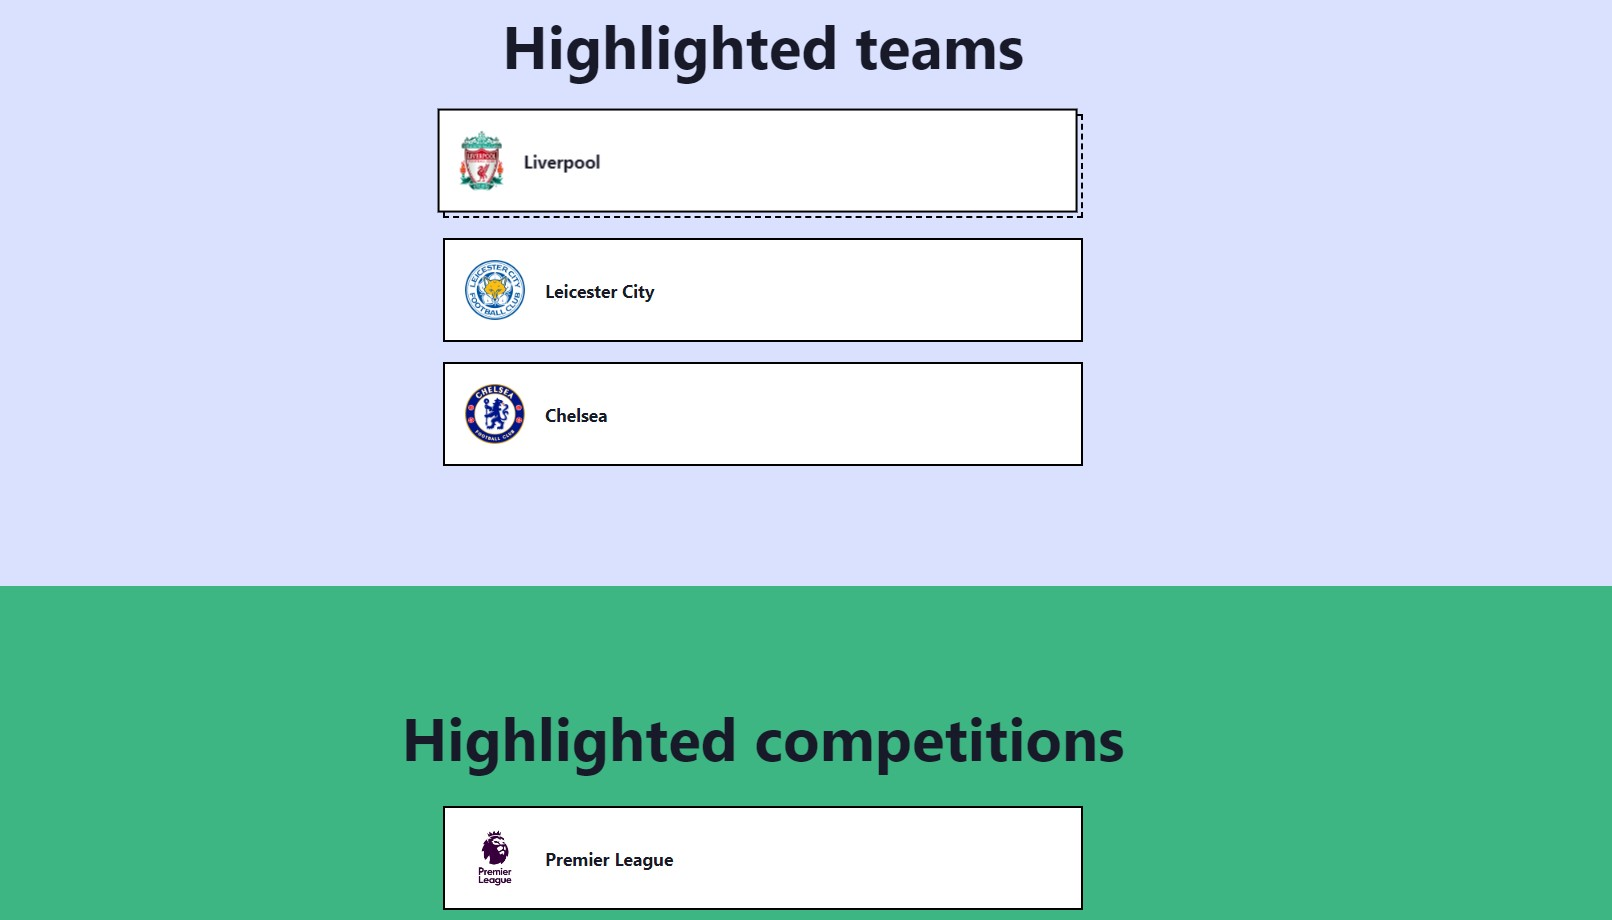
\includegraphics[width=14cm]{images/hero.jpg}
\caption{Prikaz istaknutih ekipa i natjecanja}
\label{fig:hero}
\end{figure}


\section{Autentifikacija}

Od korisnika se očekuje da bude autentificiran za samo jednu funkcionalnost, a to je spremanje omiljenih igrača i ekipa.
Korisnik koji označi nekog igrača ili ekipu kao omiljenu brže može pronaći podatke o utakmicama i statistici te ekipe ili igrača.

Svakom korisniku na navigacijskoj traci je prikazana tipka koja vodi do korisničkog profila. Ako korisnik nije prijavljen, onda aplikacija zatraži od njega da se prijavi tako da ga prebaci na odgovarajuću putanju.

Ekran za prijavu u sustav traži od korisnika korisničko ime i zaporku.

\begin{figure}[htb]
\centering
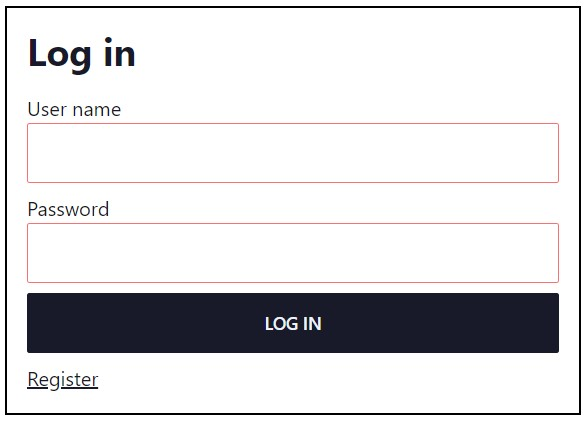
\includegraphics[width=10cm]{images/login.jpg}
\caption{Ekran prijave u sustav}
\label{fig:login}
\end{figure}

Ako korisnik unese neispravno korisničko ime ili ako predana zaporka nije točna za dano korisničko ime, onda sustav prikaže grešku gdje se navodi da nije ispravno korisničko ime ili zaporka, ali se ne kaže korisniku što točno nije ispravno.
Ako korisnik upiše ispravno korisničko ime i zaporku onda mu se dodijeli kolačić sjednice\footnote{https://www.cookieyes.com/blog/session-cookies/} i prebaci ga se na početnu stranicu aplikacije.
Kolačić sjednice se koristi da bi se nadalje znalo je li korisnik prijavljen i tko je korisnik.

Korisnik koji nema napravljen korisnički račun može prijeći na stranicu registracije preko poveznice na dnu komponente za prijavu.
Za uspješnu registraciju se od korisnika traži ime, prezime, korisničko ime te zaporka. Zaporka se mora dva puta unijeti te ako dvije unesene zaporke nisu jednake onda se korisniku ne dopušta predavanje unesenih podataka.

Prijavljeni korisnici mogu pregledati popis igrača i ekipa koje su spremili kao najdraže na stranici profila.

\begin{figure}[htb]
\centering
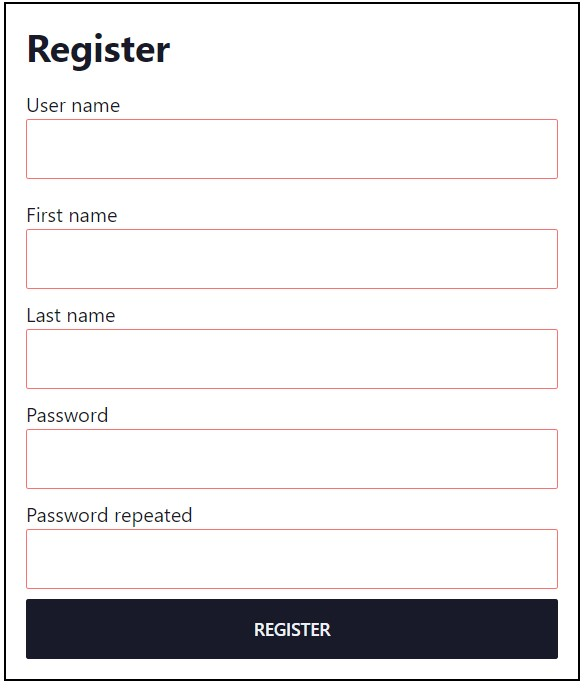
\includegraphics[width=10cm]{images/register.jpg}
\caption{Ekran registracije korisnika}
\label{fig:register}
\end{figure}

Ako korisnik unese korisničko ime koje se već koristi, onda mu korisničko sučelje prikaže da nije ispravno te da unese novo korisničko ime.
Ako su svi podatci ispravni, onda se nakon registracije automatski provede i prijava u sustav te se prebaci korisnika na početnu stranicu.

\section{Pregled utakmica}

Korisnik može doći do stranice pregleda utakmice preko navigacijske trake.

Prilikom dolaska na tu stranicu, od korisnika se traži da unese datum za koji želi pregledati utakmice. Ako korisnik nije ništa unio onda se automatski odabere datum posjećivanja stranice.
Nakon što korisnik unese željeni datum, aplikacija prikaže popis utakmica koje su igrane toga datuma uz osnovne informacije o tim utakmicama. Prikažu se ekipe koje su sudjelovale, datum i vrijeme igranja te rezultat.

\begin{figure}[htb]
\centering
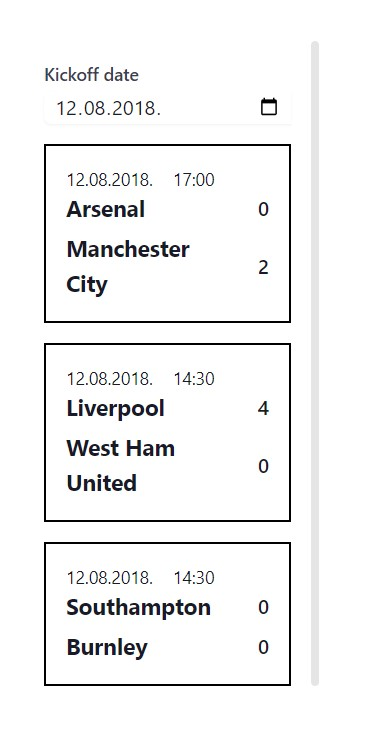
\includegraphics[width=5cm]{images/game-list.jpg}
\caption{Popis utakmica određenog datuma}
\label{fig:games-list}
\end{figure}

\subsection{Pregled detalja utakmice}

Nakon što korisnik odabere određenu utakmicu aplikacija će prikazati detalje te utakmice s desne strane popisa utakmica.
Stranica pregleda utakmica je napravljena koristeći ugniježđeno usmjeravanje (eng. nested routing)\footnote{https://start.solidjs.com/core-concepts/routing\#nested-routes}.
To znači da prilikom promjene putanje unutar aplikacije ne radimo ponovno crtanje cijelog ekrana niti učitavamo sve podatke potrebne za cijelu stranicu.
Učitavamo samo podatke koji su potrebni za prikaz onih dijelova aplikacije koji se nalaze u promijenjenom segmentu putanje.
Na stranici pregleda detalja utakmice, aplikacije ima četiri razine ugniježđenog usmjeravanja.
Prva razina se učitava za cijelu aplikaciju i ona sadrži samo navigacijsku traku i podatke o tome je li korisnik prijavljen i koju ulogu ima.
Druga razina se učitava kada se posjeti "/goals" putanju. Ta razina učitava popis dostupnih utakmica za dani datum i prikazuje ih s desne strane.
Treća razina sadrži identifikator utakmice. Tu se učitavaju osnovni podatci utakmice kao ime natjecanja i sezone u kojoj se igra utakmica, datum igranja, imena klubova, sličice grbova te rezultat.
Četvrta razina odabire jednu od tri kartice pregleda detalja utakmica: kartica s golovima, kartonima i zamjenama; kartica s grafičkim prikazom početnih jedanaest obje ekipe te kartica sa statistikom utakmice.

Ako se ne odabere niti jedna kartica na četvrtoj razini, onda aplikacija automatski prebaci korisnika na karticu s golovima utakmice.
Golovi su poredani kronološki. Pored golova, na istoj kronološkoj traci su prikazane zamjene provedene u utakmici te podijeljeni kartoni.

Ime svakog igrača prikazanog na kronološkoj traci je poveznica koja vodi na stranicu s detaljima o tome igraču.

Za svaki gol prikazano je ime igrača koji je zabio gol, ime igrača koji je asistirao za gol, minutu u kojoj je gol zabijen te rezultat utakmice nakon postignutog gola.
Ime igrača koji je zabio gol je prikazan u podebljanom fontu te se nalazi iznad imena igrača koji je asistirao za taj gol.

Svaki podijeljeni karton ima grafički prikazano je li igrač dobio žuti, crveni ili drugi žuti karton.

\begin{figure}[htb]
\centering
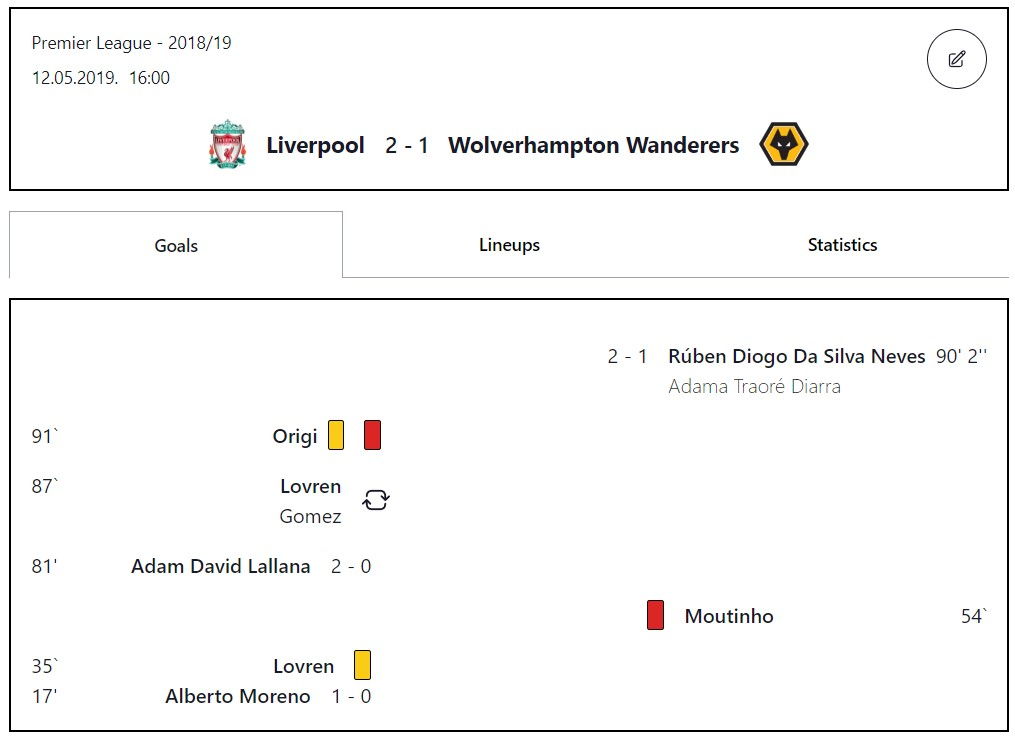
\includegraphics[width=12cm]{images/goals.jpg}
\caption{Osnovni podatci utakmice i popis golova}
\label{fig:goals}
\end{figure}

Događaji su poravnati na lijevu stranu ako je u njima sudjelovao igrač domaće ekipe, a na desnoj strani su događaji u kojima su sudjelovali igrači gostujuće ekipe.

\subsection{Prikaz statistike}

Na stranici prikaza statistike prikazuju se podatci o posjedu lopte, ukupnim udarcima, udarcima u vrata, dodavanjima, ubačajima iz kuta, driblinzima, uspješnim driblinzima, zaleđima i sl.
Osim samog broja za odgovarajuću statistiku također se grafički prikazuje omjer domaće i gostujuće ekipe.

\begin{figure}[htb]
\centering
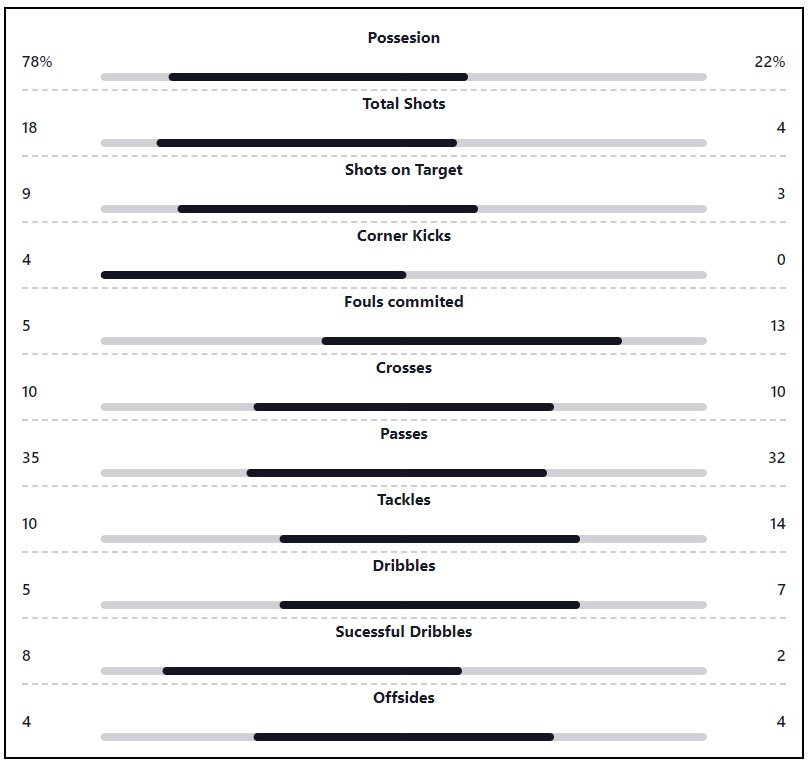
\includegraphics[width=14.2cm]{images/statistic.jpg}
\caption{Statistika utakmice}
\label{fig:statistic}
\end{figure}

\subsection{Grafički prikaz početnih jedanaest}

Svaka spremljena utakmica mora imati spremljene podatke o početnih jedanaest obije ekipe.

Ekipa može imati jednu od sljedećih početnih formacija: 442, 433, 4231, 352, 3511, 343 i 532.
Na osnovu ovog podatka te spremljenih podataka u bazi podataka grafički se prikaže izgled početnih jedanaest.

\begin{figure}[htb]
\centering
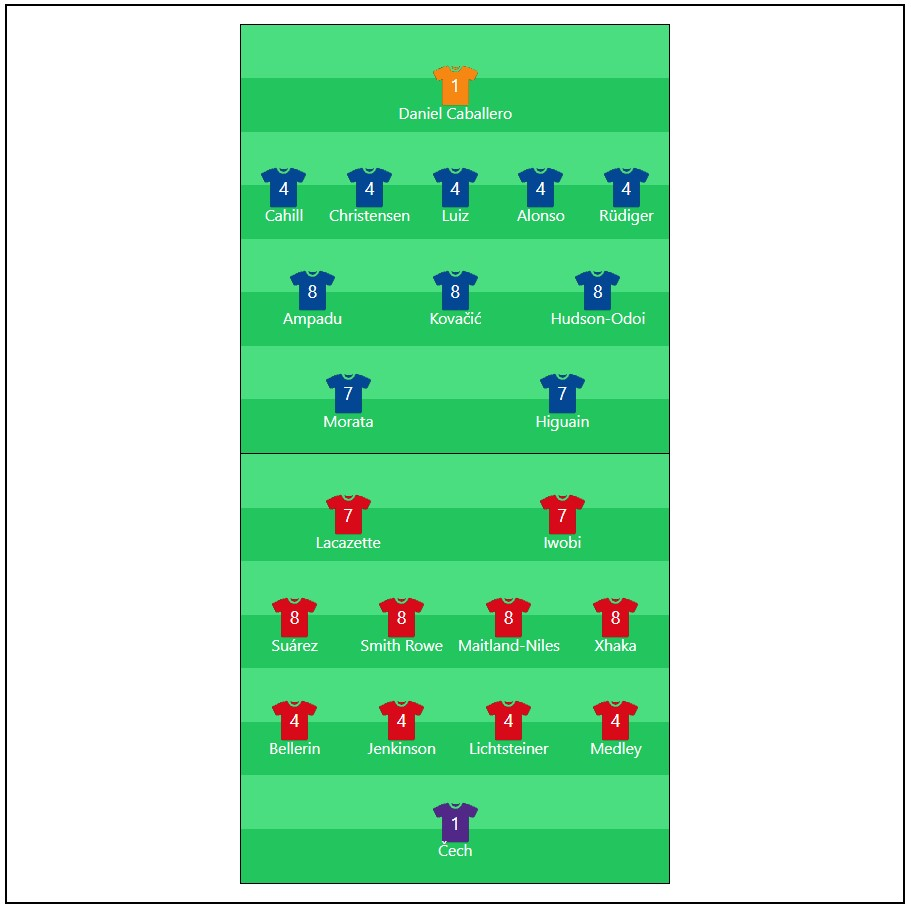
\includegraphics[width=15cm]{images/formation.jpg}
\caption{Početnih jedanaest}
\label{fig:formation}
\end{figure}

Za izradu ovog grafičkog prikaza je korišten samo CSS framework Tailwind\footnote{https://tailwindcss.com}.
Svi vidljivi elementi su ručno programirani koristeći samo dostupne tehnologije HTML-a i CSS-a. Oblik dresa je preuzet s interneta u SVG formatu te modificiran da se može mijenjati boja dresa ovisno o ekipi.
Prilikom klika na jednog od igrača, korisnika se odvede na stranicu pregleda detalja tog igrača.

Prikaz početne postave se sastoji od jednog HTML elementa koji služi kao roditelj ostalih te on sadrži samo crni rub.
Unutar njega su naslagani elementi zelene pozadinske boje. Zeleni elementi su poredani da se izmjenjuju tamnija i svjetlija nijansa zelene boje.

Nakon zelenih traka dolaze dva bloka redova igrača. Ova dva bloka su unutar jednog elementa koji služi kao roditelj i ima apsolutnu poziciju što omogućava da su redovi igrača nacrtani preko zelenih traka.
Dva bloka redova igrača imaju istu logiku crtanja pozicija igrača, ali drugi blok ima Tailwind klasu "flex-col-reversed" što znači da red s vratarom, koji se treba prikazati prvi, se zapravo prikaže zadnji.

U slučaju kada ne postoje podatci početnih postava, ili ako podatci početnih postava nisu ispravni, tada se korisniku prikaže poruka da je došlo do greške te se prikaže popis svih igrača koji su igrali za
domaću i gostujuću ekipu te sezone.

\begin{figure}[htb]
\centering
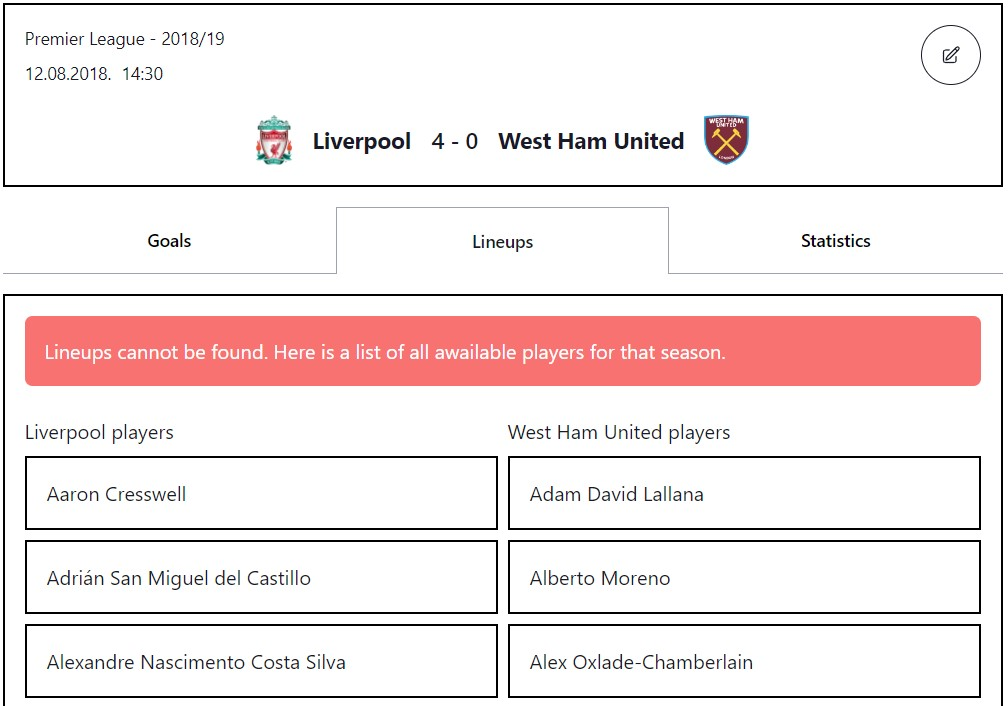
\includegraphics[width=14.2cm]{images/lineup-fallback.jpg}
\caption{Početnih jedanaest}
\label{fig:formation}
\end{figure}


\subsection{Uređivanje podataka utakmice}

Korisnik koji ima ulogu administratora može pristupiti stranici uređivanja podataka postojeće utakmice i stranici stvaranja nove utakmice.
Poveznica na stranicu stvaranje nove utakmice je vidljiva administratoru na navigacijskoj traci, a poveznica na stranicu uređivanja postojeće utakmice se nalazi na prikazu detalja utakmice.

\begin{figure}[htb]
\centering

\includegraphics[width=14cm]{images/navigation.jpg}
\caption{Navigacijska traka}
\label{fig:formation}
\end{figure}


Od korisnika se prvo traži da unese željeno natjecanje u kojemu se igra utakmica te jednu od dostupnih sezona za to natjecanje.
Nakon odabira natjecanja i sezone, učita se popis svih ekipa koje su sudjelovale te sezone u tome natjecanju.
Od korisnika se traži da odabere ekipu domaćina i gostujuću ekipu. Nakon toga se učitaju svi igrači i izbornici koji su bili članovi odabranih ekipa te sezone.

Vrijeme početka utakmice se unosi kroz HTML ulazno polje koje ime vrstu "datetime-local\footnote{https://developer.mozilla.org/en-US/docs/Web/HTML/Element/input/datetime-local}".
To ulazno polje traži od korisnika da unese datum te u koliko sati počinje utakmica.

Status utakmice i treneri dviju ekipa se biraju kroz padajući izbornik, dok se početne postave ekipa biraju kroz posebno grafičko sučelje.
S desne strane pretpregleda početnih postava prikazan je padajući izbornik formacija početnih postava te izbornik boje dresova vratara i igrača dviju ekipa.
Pregled početnih postava ekipa je prilagođen da odabirom određene pozicije ili igrača se otvori izbornik gdje korisnik mora odabrati jednog igrača te broj koji će biti prikazan na njegovom dresu.

\begin{figure}[htb]
\centering
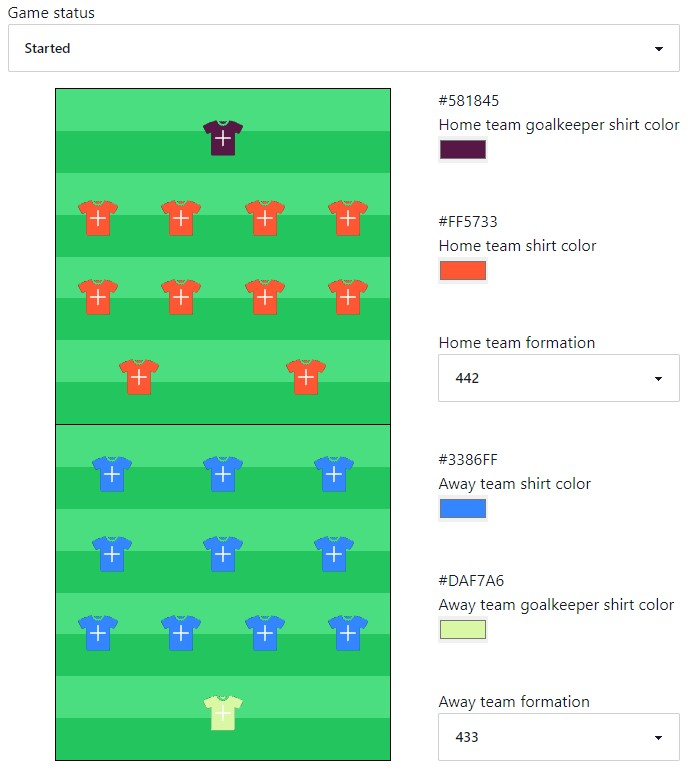
\includegraphics[width=12cm]{images/edit-game.jpg}
\caption{Uređivanje početnih postava}
\label{fig:formation}
\end{figure}

Ispod toga se nalazi sučelje za dodavanje i uređivanje golova, kartona i zamjena utakmice.
Nakon dodavanja gola, kartona ili zamjene, taj događaj se prikaže u pretpregledu kronološki poredano kao što se bi se prikazalo na stranici pregleda detalja utakmice.
Pored svakog dodanog događaja na utakmici prikazana je tipka koja uklanja taj događaj s utakmice.

Ako je korisnik za status utakmice odabrao bilo koji status, osim onoga koji označava da utakmica nije započela, onda je prikazano sučelje uređivanja statistike utakmice.
Prikazani su pretpregledi statistike kao na stranici pregleda detalja utakmice, ali je iznad svake stavke prikazana komponenta za unos pojedinog podatka za domaću i gostujuću ekipu.

Ako su svi uneseni podatci ispravni, onda se korisniku omogući spremanje podataka te utakmice. Nakon uspješnog spremanja podataka utakmice pošalje se WebSocket poruka da su podatci te utakmice ažurirani.
Ako se u tom trenutku neki korisnik nalazi na stranici pregleda detalja te utakmice, onda se invalidiraju svi podatci te putanje. Tako je osigurano ažuriranje podataka detalja utakmice u stvarnom vremenu.

Pošto je aplikacija podignuta na bezposlužiteljskoj okolini, nije moguće pokrenuti vlastiti WebSocket poslužitelj.
Zbog toga je za izradu WebSocket komunikacije korišten servis Pusher\footnote{https://pusher.com/} koji prihvati poruku od Node servera.
Pusher nakon toga pošalje WebSocket poruku svim pretplatnicima na određeni kanal.
Korisnik se automatski pretplati na WebSocket kanal dolaskom na stranicu pregleda detalja neke utakmice te se pretplata automatski otkaže kada ode s te stranice.

\section{Pregled detalja igrača i trenera}

Pregled i ažuriranje podataka igrača i trenera su dosta slični. Pregled detalja igrača i trenera se sastoji od slike, prikaza osobnih podataka, te trenutne ekipe za koju taj igrač igra, tj. koju taj trener trenira.

\begin{figure}[htb]
\centering
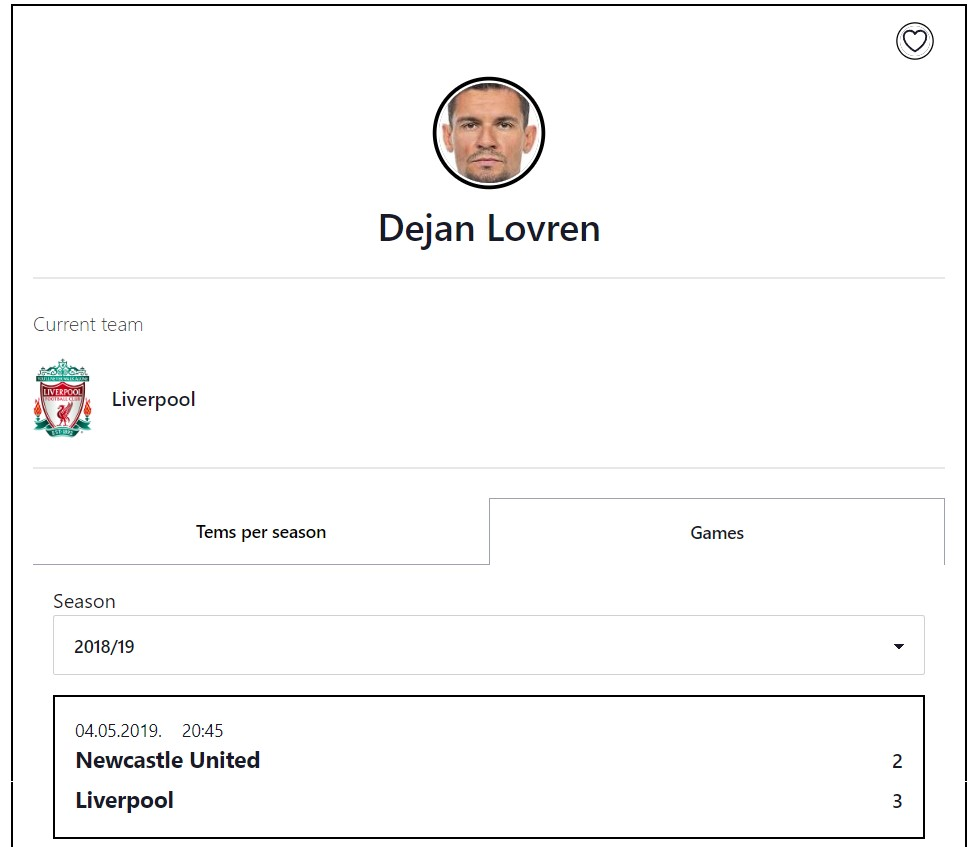
\includegraphics[width=12cm]{images/lovren.jpg}
\caption{Pregled detalja igrača}
\label{fig:player}
\end{figure}

Ispod osnovnih podataka se nalaze dvije kartice. Prva kartica prikazuje popis ekipa po sezoni za koje je taj igrač igrao ili koje je taj trener trenirao.
Druga kartica prikazuje popis utakmica u kojima je igrač igrao u početnoj postavi. Ako se nalazimo na pregledu trenera, onda je to popis utakmica u kojema je on bio trener domaće ili gostujuće ekipe.

Stranica pregleda detalja igrača sadrži i tipku pomoću koje se dodaje ili uklanja igrača s popisa najdražih. Ako korisnik koji nije prijavljen klikne na tu tipku, onda ga se prebaci na stranicu prijave.

Prijavljeni korisnici koji imaju ulogu administratora mogu uređivati podatke igrača i trenera preko dvije poveznice.
Jedna poveznica odvodi na stranicu gdje se uređuju osnovni podatci kao ime, prezime, slika, datum rođenja i trenutna ekipa.
Druga poveznica odvodi na stranicu gdje se unose podatci za koju je ekipu taj igrač igrao, tj. koju je ekipu taj trener trenirao, u određenoj sezoni.
Ta se stranica sastoji od popisa gdje svaki redak ima padajući popis ekipa, padajući popis sezona te tipku koja uklanja trenutni redak.
A na dnu te stranice se nalazi tipka koja dodaje novi redak i tipka koja sprema podatke.

\begin{figure}[htb]
\centering
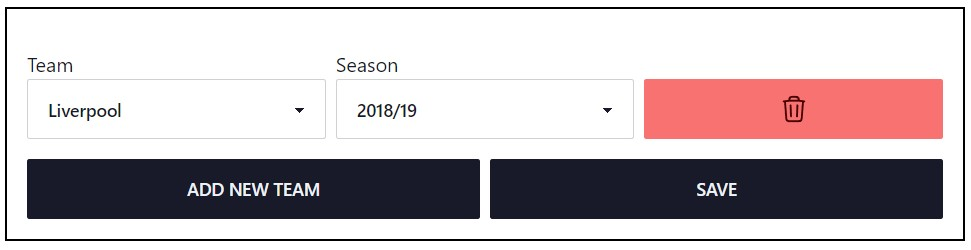
\includegraphics[width=14cm]{images/per-season.jpg}
\caption{Uređivanje podataka o ekipama po sezoni}
\label{fig:per-season}
\end{figure}

\newpage
\section{Pregled detalja ekipe}

Pregled detalja ekipe se sastoji osnovnih podataka ekipe kao ime, slika grba te slika države iz koje dolazi ta ekipa.

\begin{figure}[htb]
\centering
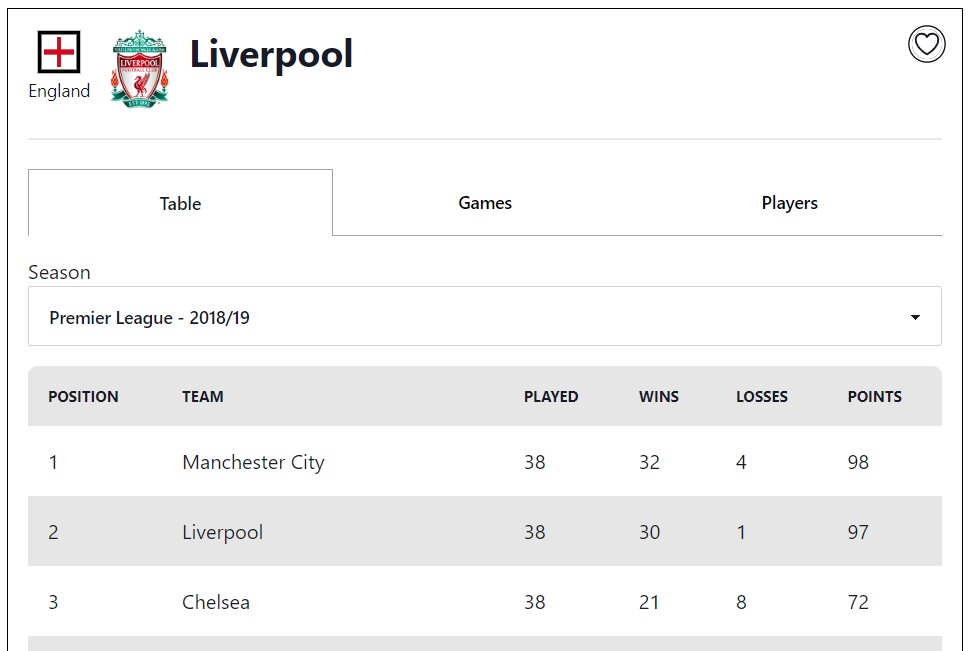
\includegraphics[width=14cm]{images/team.jpg}
\caption{Prikaz detalja ekipe}
\label{fig:per-season}
\end{figure}

Ispod toga se nalaze tri kartice. Prva kartica prikazuje tablicu poretka u natjecanjima u kojima je sudjelovala ta ekipa. Na vrhu je dostupan padajući izbornik natjecanja i sezona u kojima je sudjelovala ekipa.
Ime svake ekipe služi kao poveznica koja vodi na stranicu detalja te ekipe.
Druga kartica prikazuje popis utakmica po sezonama i natjecanjima u kojima je sudjelovala ekipa s padajućim izbornikom natjecanja i sezona. Odabirom određene utakmice korisnika se prebacuje na prikaz detalja te utakmice.
Treća kartica prikazuje popis igrača po sezonama koji su igrali za tu ekipu.

\section{Pretraga igrača, trenera i ekipa}

Korisnik klikom na tipku s ikonom povećala na navigacijskoj traci dobije polje za unos pojma pretrage. Nakon unosa pojma pretrage korisnika se vodi na stranicu rezultata pretrage.
Prikazuju se pronađeni rezultati za igrače, trenere i ekipe.
Kod igrača i trenera, pretraga se vrši tako da se usporedi sadrži li ime ili prezime osobe uneseni pojam kao podniz.
Razlika velikih i malih slova se ignorira. Kod pretrage ekipa provjerava se samo sadrži li ime ekipe uneseni pojam kao podniz.

Rezultati pretrage se prikazuju u tri stupca. Jedan stupac je za igrače, jedan za trenere i jedan za ekipe. Za sva tri entiteta se prikaže ime i slika ako je dostupna.

\begin{figure}[htb]
\centering
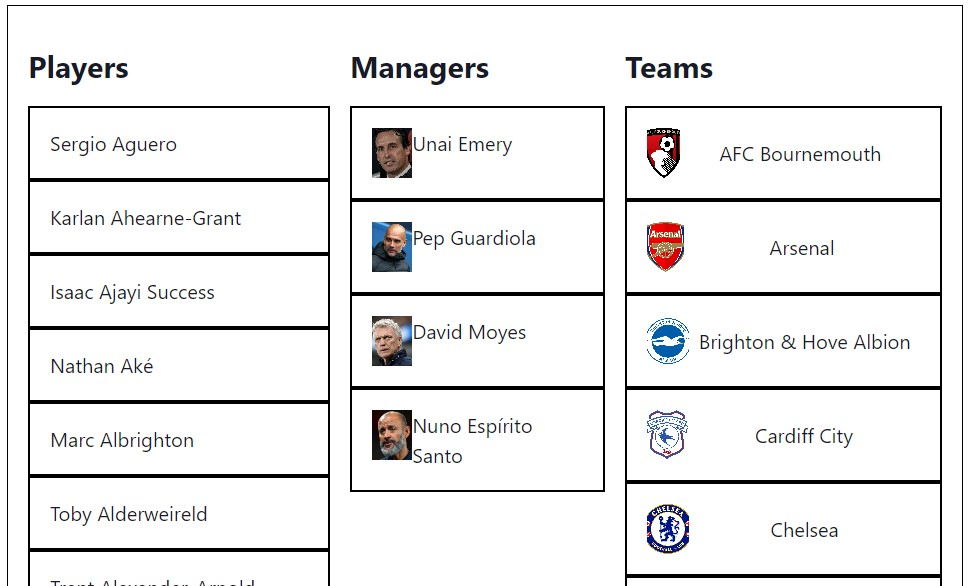
\includegraphics[width=14cm]{images/search.jpg}
\caption{Rezultati pretrage}
\label{fig:search}
\end{figure}

\section{Pregled detalja natjecanja}

Kod pregleda detalja određenog natjecanja prikazani su ime natjecanja, slika i ime države u kojoj se održava natjecanje te grb natjecanja ako postoji.

Ispod osnovnih informacija o natjecanju prikazane su dvije kartice koje prikazuju popis utakmica odigranih po određenoj sezoni te tablica poretka ekipa koje su sudjelovale u tome natjecanju određene sezone.
U oba slučaja se identifikator sezone sprema u putanji URL-a te ako korisnik slučajno dođe na stranicu pregleda tablice ili popisa utakmica bez identifikatora određene sezone, aplikacija će automatski preusmjeriti korisnika na najnoviju dostupnu sezonu toga natjecanja.

Tablica poretka se ne sprema u bazi podataka nego se izračuna svaki put kada se čita.
Učita se popis svih utakmica za tu sezonu, napravi se mapa koja mapira identifikator ekipe na objekt koji sadrži podatke o bodovima ekipe, broju odigranih utakmica, broju pobjeda, broju gubitaka te broju neriješenih utakmica.
Prolazi se kroz popis utakmica te se ažurira objekt koji sadrži podatke za domaću i gostujuću ekipu.
Entitet utakmice ne bilježi tko je pobjednik, nego se to izračuna na osnovu zabijenih golova na utakmici. Prebroje se golovi i autogolovi te se na osnovu toga odredi tko dobiva tri, jedan ili nula bodova.

\begin{figure}[htb]
\centering
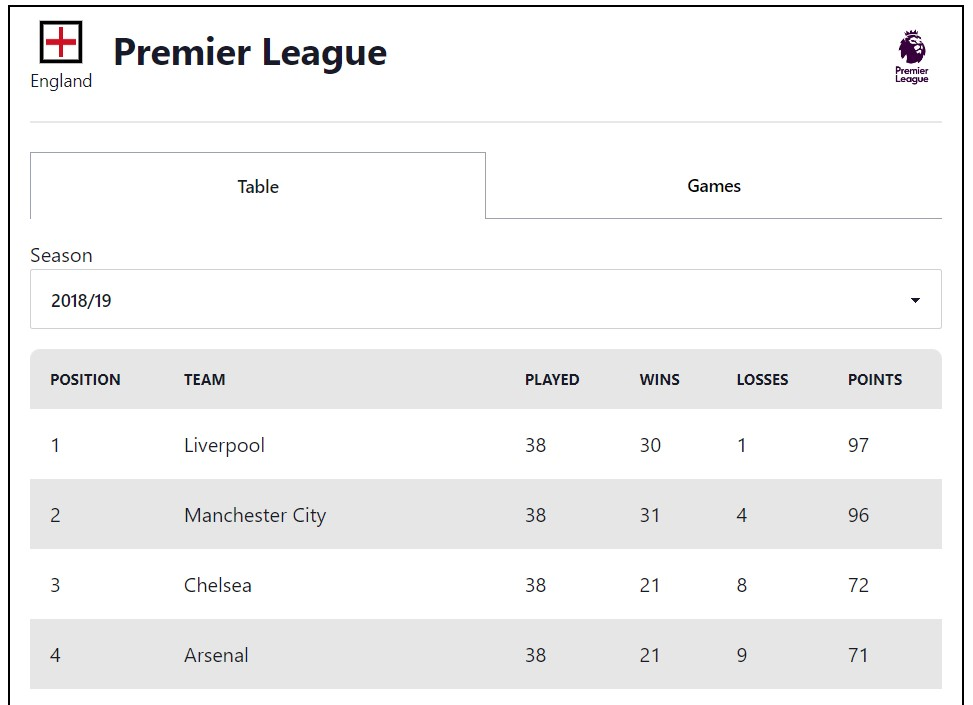
\includegraphics[width=14cm]{images/table.jpg}
\caption{Tablica poretka ekipa}
\label{fig:table}
\end{figure}

\chapter{Zaključak}

Izradom ove aplikacije uspješno je omogućeno lako pregledavanje detalja odigranih nogometnih utakmica.
Korisniku je omogućeno brzo i lako pretraživanje dostupnih igrača, trenera i ekipa.

Stranice koje prikazuju podatke povezanog resursa sadržavaju poveznice koje vode korisnika na stranicu pregleda detalja tog resursa.
Za entitete koji sadrže jako malo informacija, kao sezona koja sadrži samo naziv, nije napravljena mogućnost uređivanja niti unosa novih podataka jer se ti podatci ne ažuriraju često i lako ih je dodati direktno kroz bazu podataka.
Napravljena su sučelja za uređivanje podataka o utakmicama, igračima i trenerima te unos novih podataka.
Omogućen je lak odabir povezanih resursa pri uređivanju podataka preko padajućih izbornika.

Najveći izazov je bila izrada grafičkog prikaza i uređivanja početnih postava i formacija ekipa neke utakmice.
Cijeli grafički prikaz i uređivanje početnih postava izrađeno je koristeći isključivo CSS framework Tailwind i JavaScript framework SolidJs.

Sve forme za uređivanje podataka na stranici, osim one za uređivanje podataka određene utakmice, napravljene su oslanjajući se na HTML form element poboljšan SolidStart-ovim \emph{createServerAction\$()}.
Uređivanje podataka o početnim postavama je bilo previše komplicirano pa se taj podatak šalje kao JSON.
Kao poboljšanje bi se moglo napraviti da se prikaz svakog igrača u početnoj postavi sastoji od par skrivenih \emph{input} polja koja se popune s potrebnim vrijednostima, kao identifikator odabranog igrača i broj na leđima,
nakon ispunjavanja pomoćne forme koja bi se otvorila u lebdećem prozoru nakon odabira određene pozicije u početnoj postavi.

Pisanjem aplikacije u fullstack framework-u povećana je brzina izrade funkcionalnih zahtjeva.
SolidStart meta-framework omogućio je pisanje koda koji se izvodi isključivo na poslužitelju unutar klijentskih komponenti čime se dobiva osjećaj pisanja desktop aplikacije.
Dohvat podataka se vrši samo pozivanjem funkcije. Programer ne mora razmišljati o odvajanju poslužiteljskog i klijentskog koda, otvaranju HTTP endpointa te mapiranju parametara koji se šalju preko HTTP zahtjeva.

\bibliography{literatura}
\bibliographystyle{fer}

\begin{sazetak}
Ovaj završni rad opisuje proces izrade web-aplikacije za praćenje nogometnih rezultata.
U prvom poglavlju je odrađena analiza postojećih rješenja na internetu.
Nakon toga je opisan plan izrade projekta te glavne funkcionalnosti izdvojene iz postojećih pronađenih rješenja.
Dalje slijedi model podataka, opis arhitekture aplikacije te proces izrade aplikacije.
Arhitektura aplikacije opisuje odabrane tehnologije za izradu aplikacije te platforme na kojima je aplikacija i baza podataka podignuta.
Proces izrade aplikacije opisuje svaku cjelinu za koju je napravljeno sučelje za pregled ili uređivanje podataka.

\kljucnerijeci{web, solidjs, nodejs, postgress, nogomet}
\end{sazetak}

% TODO: Navedite naslov na engleskom jeziku.
\engtitle{A Web Application for Statistics Tracking of Football Matches}
\begin{abstract}
This thesis describes the process of creating a web application for tracking football results.
The first chapter contains the analysis of existing solutions on the Internet.
After that comes the description of the project development plan and the main functionalities found on existing solutions.
Next follows the data model, the description of the application architecture and the process of creating the application.
The application architecture describes the selected technologies for creating the application and the platform on which the application and database are built.
The application creation process describes each entity for which an interface for viewing or editing data has been created.

\keywords{web, solidjs, nodejs, postgress, football}
\end{abstract}

\end{document}
